\section{Word Embeddings}

I chose to do this part using the Frensh embeddings
since I know some French.

\begin{problem}[1]
  Get the $25$ most similar words to the words for man (\emph{homme})
  and woman (\emph{femme}) in the language you are working with.

  \begin{answer}
    Although the word embeddings are very high-dimensional
    (in this case, $300$), the embeddings for \emph{man}
    and \emph{woman} are very close, and each shows up in the
    top $25$ most similar words to the other.
  \end{answer}

  % screenshots
  \begin{figure}[H]
    \centering
    \begin{minipage}[b]{\textwidth}
      \centering
      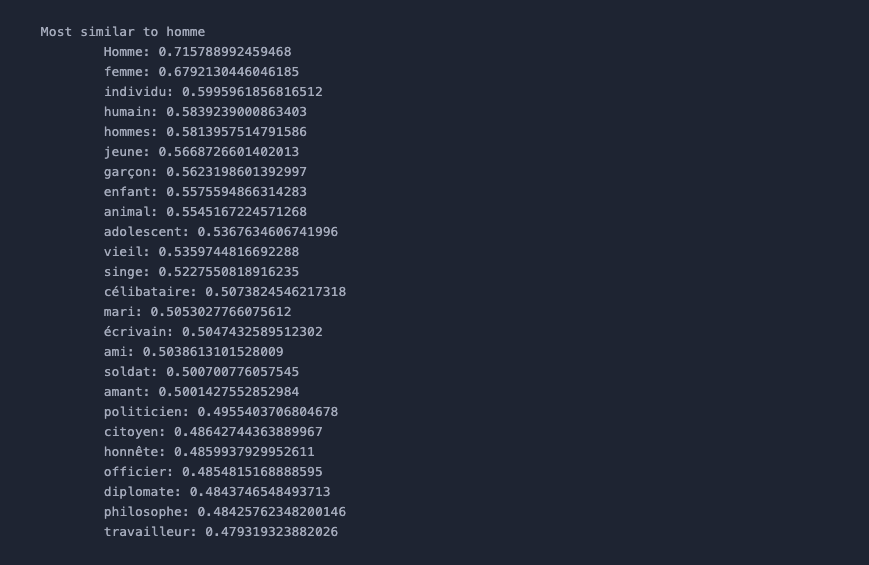
\includegraphics[width=\textwidth]{figures/3-homme-similar.png}
      \caption{Words Closest to Homme}
      \label{fig:word-embeddings-1}
    \end{minipage}
  \end{figure}
  \begin{figure}[H]
    \begin{minipage}[b]{\textwidth}
      \centering
      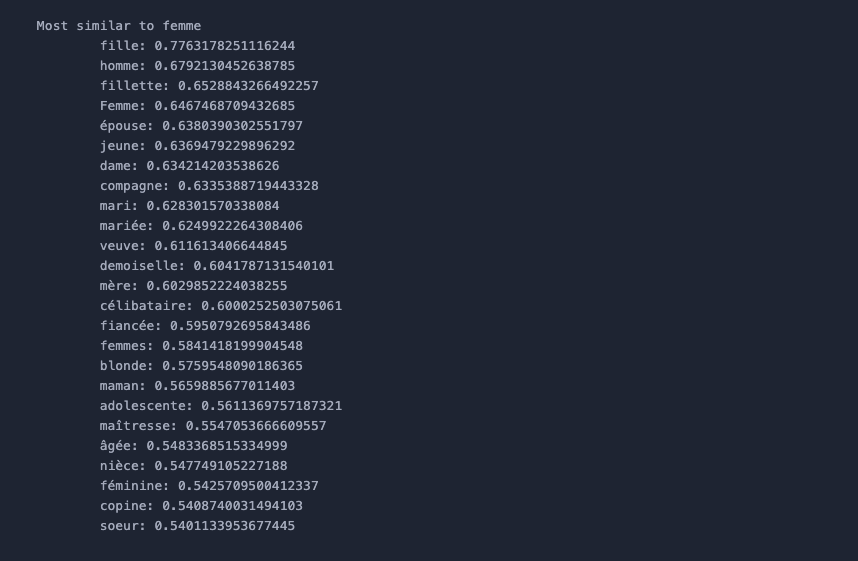
\includegraphics[width=\textwidth]{figures/3-femme-similar.png}
      \caption{Words Closest to Femme}
      \label{fig:word-embeddings-2}
    \end{minipage}
  \end{figure}

  \begin{answer}
    We also notice words that are semantically related to each of these
    showing up among the top natches:
    
    \textbf{Notable Top-Matches for \emph{Homme} (Man)}
    \begin{itemize}
      \item \emph{humain} (`human')
      \item \emph{individu} (`individual')
      \item \emph{jeune} (`young')
      \item \emph{mari} (`husband')
    \end{itemize}
  
    \textbf{Notable Top-Matches for \emph{Femme} (Woman)}
    \begin{itemize}
      \item \emph{fille} (`girl')
      \item \emph{\'epouse} (`wife')
      \item \emph{dame} (`lady')
      \item \emph{maman} (`mom')
    \end{itemize}
  \end{answer}
\end{problem}

\newpage
\begin{problem}
  Try to perform the arithmetic \crim{$\qquad \text{king} - \text{man} + \text{woman} \qquad$}
  in your language.

  \begin{figure}[H]
    \centering
    \begin{minipage}[b]{0.8\textwidth}
      \centering
      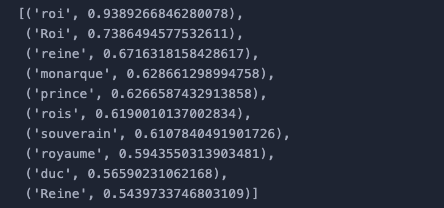
\includegraphics[width=0.9\textwidth]{figures/3-arithmetic.png}
      \caption{\crim{$\qquad \text{king} - \text{man} + \text{woman} \qquad$}}
      \label{fig:word-arithmetic}
    \end{minipage}
  \end{figure}

  \begin{answer}
    We notice words such as \emph{reine} (`queen')
    among the top matches, a good sign that the arithmetic is working
    as expected. We al;so notice other words associated with royalty
    and nobility among the top matches.

    \textbf{Notable matches}
    \begin{itemize}
      \item \emph{reine} (`queen')
      \item \emph{monarque} (`royal')
      \item \emph{souverain} (`sovereign')
      \item \emph{royaume} (`kingdom')
      \item \emph{duc} (`duke')
    \end{itemize}
  \end{answer}
\end{problem}

\newpage
\begin{problem}
  Print the \verb|t-SNE| chart for the words for
  \begin{itemize}
    \item $\text{man} \mapsto \crim{\text{homme}}$
    \item $\text{woman} \mapsto \crim{\text{femme}}$
    \item $\text{king} \mapsto \crim{\text{roi}}$
    \item $\text{queen} \mapsto \crim{\text{reine}}$
    \item $\text{child} \mapsto \crim{\text{enfant}}$
    \item $\text{boy} \mapsto \crim{\text{gar\c{c}on}}$
    \item $\text{girl} \mapsto \crim{\text{fille}}$
  \end{itemize}
  in the language that you’ve chosen.
  I recommend that you use the functions \verb|TSNE| from \verb|sklearn|
  and \verb|pyplot| from \verb|matplotlib|.



  \begin{figure}[H]
    \centering
    \begin{minipage}[b]{0.8\textwidth}
      \centering
      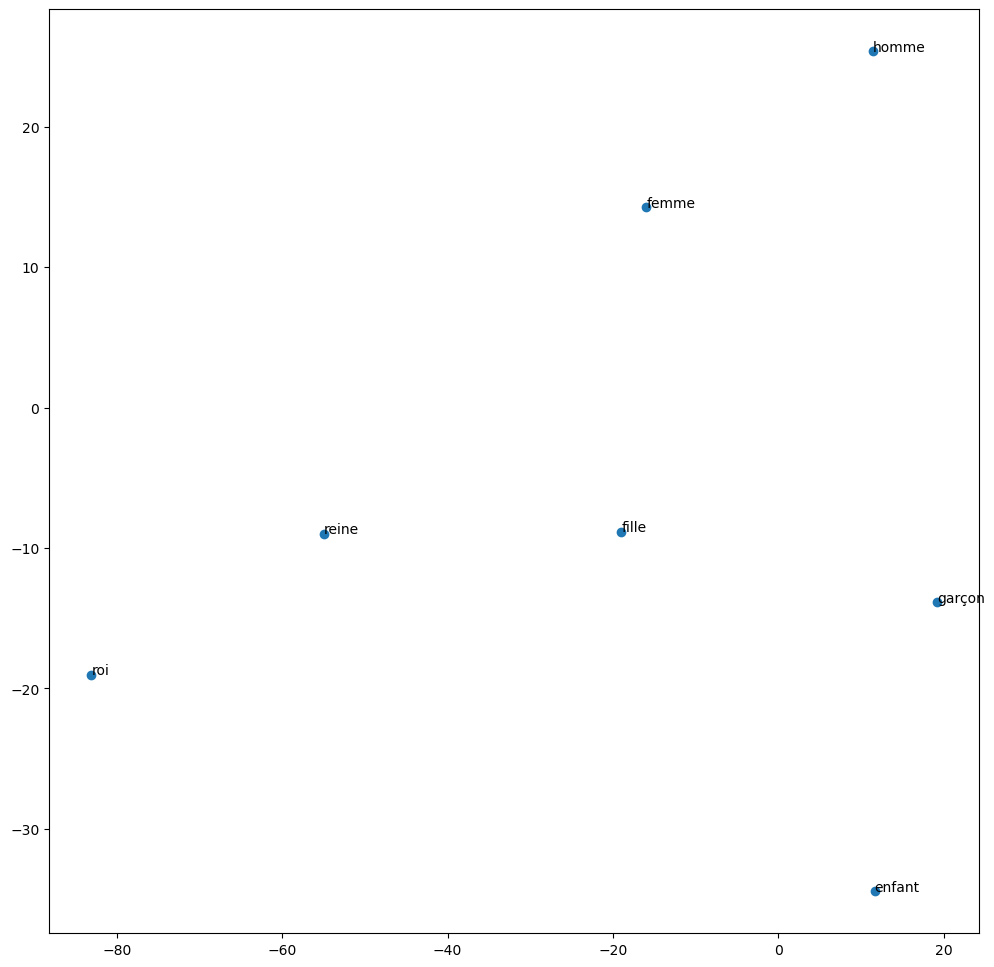
\includegraphics[width=\textwidth]{figures/3-tsne.png}
      \caption{TSNE Chart}
      \label{fig:tsne-chart}
    \end{minipage}
  \end{figure}

  \newpage
  \begin{answer}
    We notice similarities in the relations between embeddings.
    \begin{itemize}
      \item The separation between \verb|homme| and \verb|garcon| is similar
        to the separation between \verb|femme| and \verb|fille|.
      \item The separation between \verb|roi| and \verb|reine| is similar
        to the separation between \verb|homme| and \verb|femme|
        However, this separation seems inverted. Why's that?
        I think it might be an issue with how the reduction of dimensions
        is done, since I would expect \verb|roi| and \verb|reine|
        to be in the swapped positions.
      \item The separation between \verb|garcon| and \verb|fille|
        is comparable to the separation between \verb|homme| and \verb|femme|
        on the $X$-axis. However, \verb|fille| is higher up on the $Y$-axis
        than expected. This might be a result of it being used in other contexts
        where its association with someone being `young' is less pronounced.
    \end{itemize}
  \end{answer}
\end{problem}
